
\noindent 5. (\textbf{CLRS 8.2-1}) Simule a execução do $\proc{CountingSort}$ 
usando como entrada o vetor:
\[ A[1 \cdots 11] = \langle6, 0, 2, 0, 1, 3, 4, 6, 1, 3, 2\rangle  \]
\\ [6pt]
\textbf{Resposta:} A configuração inicial do algoritmo após o laço inicial será:
\begin{figure}[h]
  \centering
    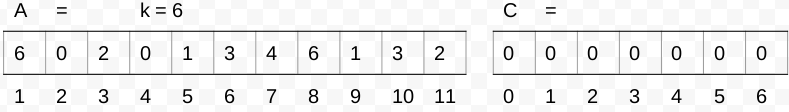
\includegraphics[width=0.8\textwidth]{q5-5-p1}
\end{figure}
\\
O vetor $A$ nunca é alterado, o vetor $C$ é representado abaixo após o final do 
segundo laço (esquerda) e após o final do terceiro laço (direita):
\begin{figure}[h]
  \centering
    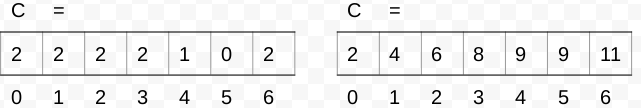
\includegraphics[width=0.8\textwidth]{q5-5-p2}
\end{figure}
\\
O último laço começa pelo com o índice $j = n$ e vai até 1, o vetor B começa 
vázio e vai sendo preenchido até o final do algoritmo. Abaixo segue os estados 
dos vetores $C$ e $B$ no fim das iterações $j = 8, j = 4$ e $j = 1$:
\begin{figure}[h]
  \centering
    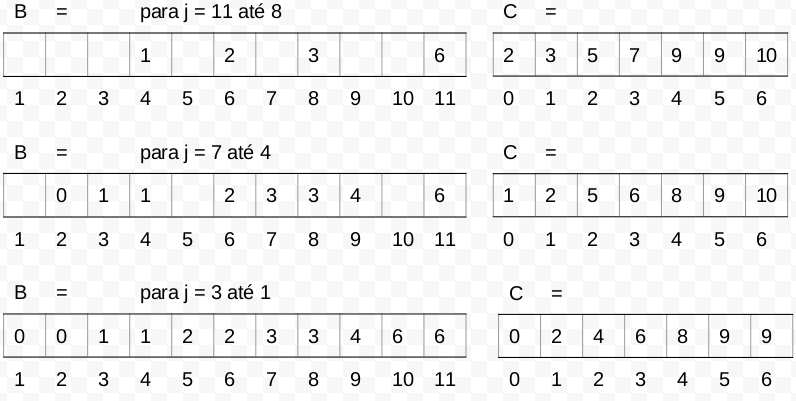
\includegraphics[width=0.8\textwidth]{q5-5-p3}
\end{figure}
\\
Então o algoritmo se encerra mantendo o vetor $B$ ordenado.
\\[12pt]
